\begin{frame}{Why Parallel?}
  \begin{itemize}
  \item Solve a fixed problem faster
  \item Obtain a more accurate solution in the same amount of time
  \item Solve a more complicated problem in the same amount of time
  \item Use more memory than available on one machine
  \end{itemize}
\end{frame}

\begin{frame}{Strong Scaling}
  \begin{center}
    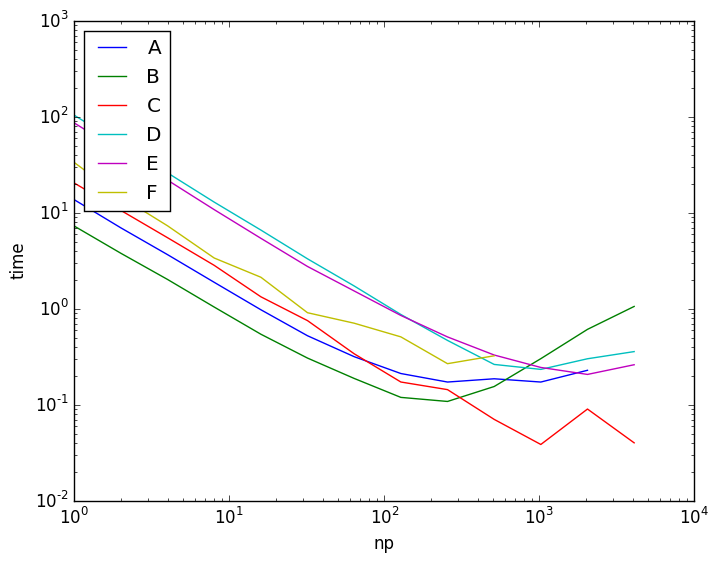
\includegraphics[width=.8\textwidth]{figures/olenz/olenz-time-np}
  \end{center}
  \begin{itemize}
  \item Good: shows absolute time
  \item Bad: log-log plot makes it difficult to discern efficiency
    \begin{itemize}
    \item Stunt 3: \url{http://blogs.fau.de/hager/archives/5835}
    \end{itemize}
  \end{itemize}
\end{frame}

\begin{frame}{Efficiency versus Number of Processes}
  \begin{center}
    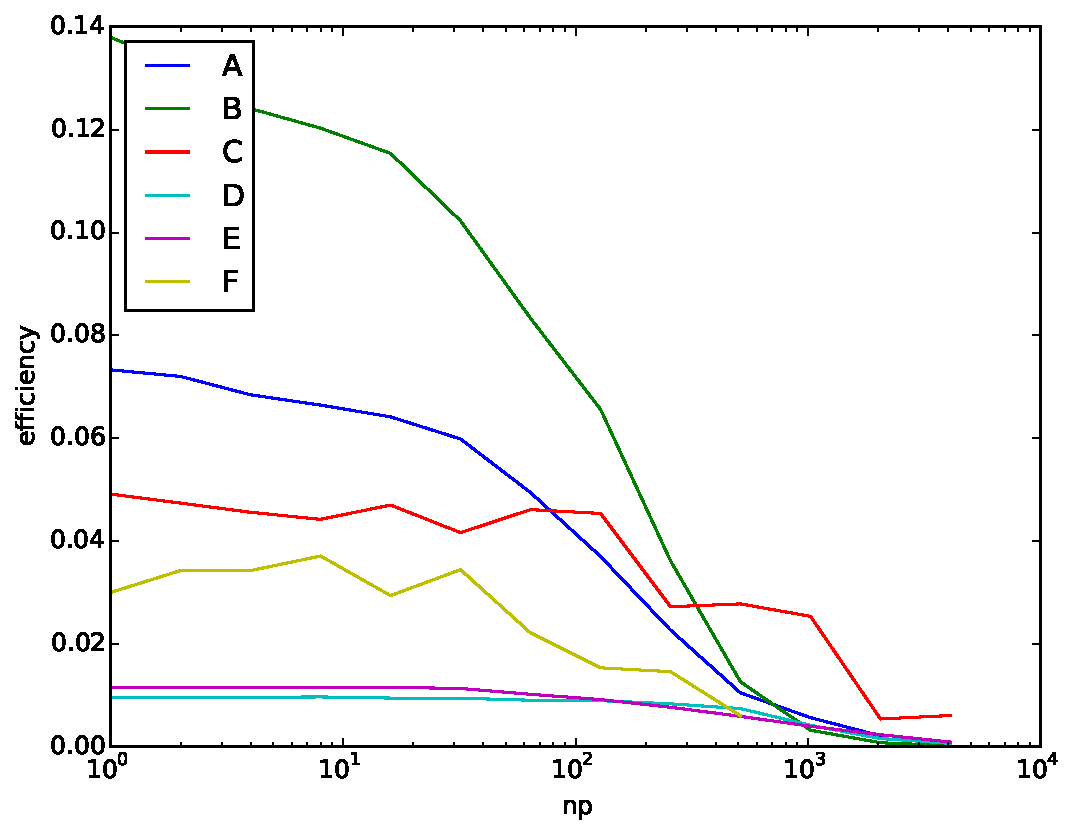
\includegraphics[width=.8\textwidth]{figures/olenz/olenz-efficiency-np}
  \end{center}
  \begin{itemize}
  \item Good: shows efficiency at scale
  \item Bad: no absolute time
  \end{itemize}
\end{frame}

\begin{frame}{Efficiency versus Time}
  \begin{center}
    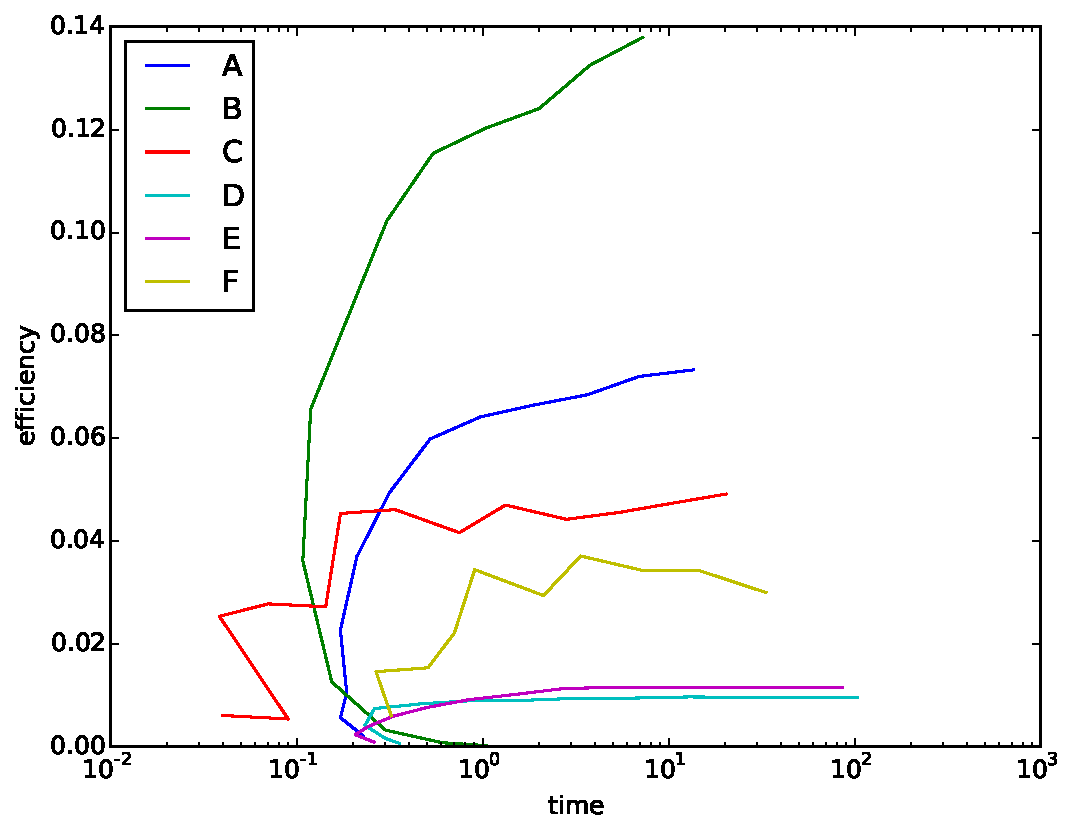
\includegraphics[width=.8\textwidth]{figures/olenz/olenz-efficiency-time}
  \end{center}
  \begin{itemize}
  \item Good: absolute time
  \item Good: efficiency (preferably with units, like DOF/s/process)
  \item Bad: harder to see machine size (but less important)
  \end{itemize}
\end{frame}

\begin{frame}{Scaling Challenges}
  \begin{quote} \centering
    The easiest way to make software scalable \\
    is to make it sequentially inefficient. \\
    (Gropp 1999)
  \end{quote}
  \begin{itemize}
  \item Solver iteration count may increase from
    \begin{itemize}
    \item increased resolution
    \item model parameters (e.g., coefficient contrast/structure)
    \item more realistic models (e.g., plasticity)
    \item model coupling
    \end{itemize}
  \item Algorithm may have suboptimal complexity (e.g., direct solver)
  \item Increasing spatial resolution requires more time steps (usually)
  \item Implementation/data structures may not scale
  \item Architectural effects -- cache, memory
  \end{itemize}
\end{frame}

\begin{frame}{Accuracy-time tradeoffs: \emph{de rigueur} in ODE community}
  \begin{center}
    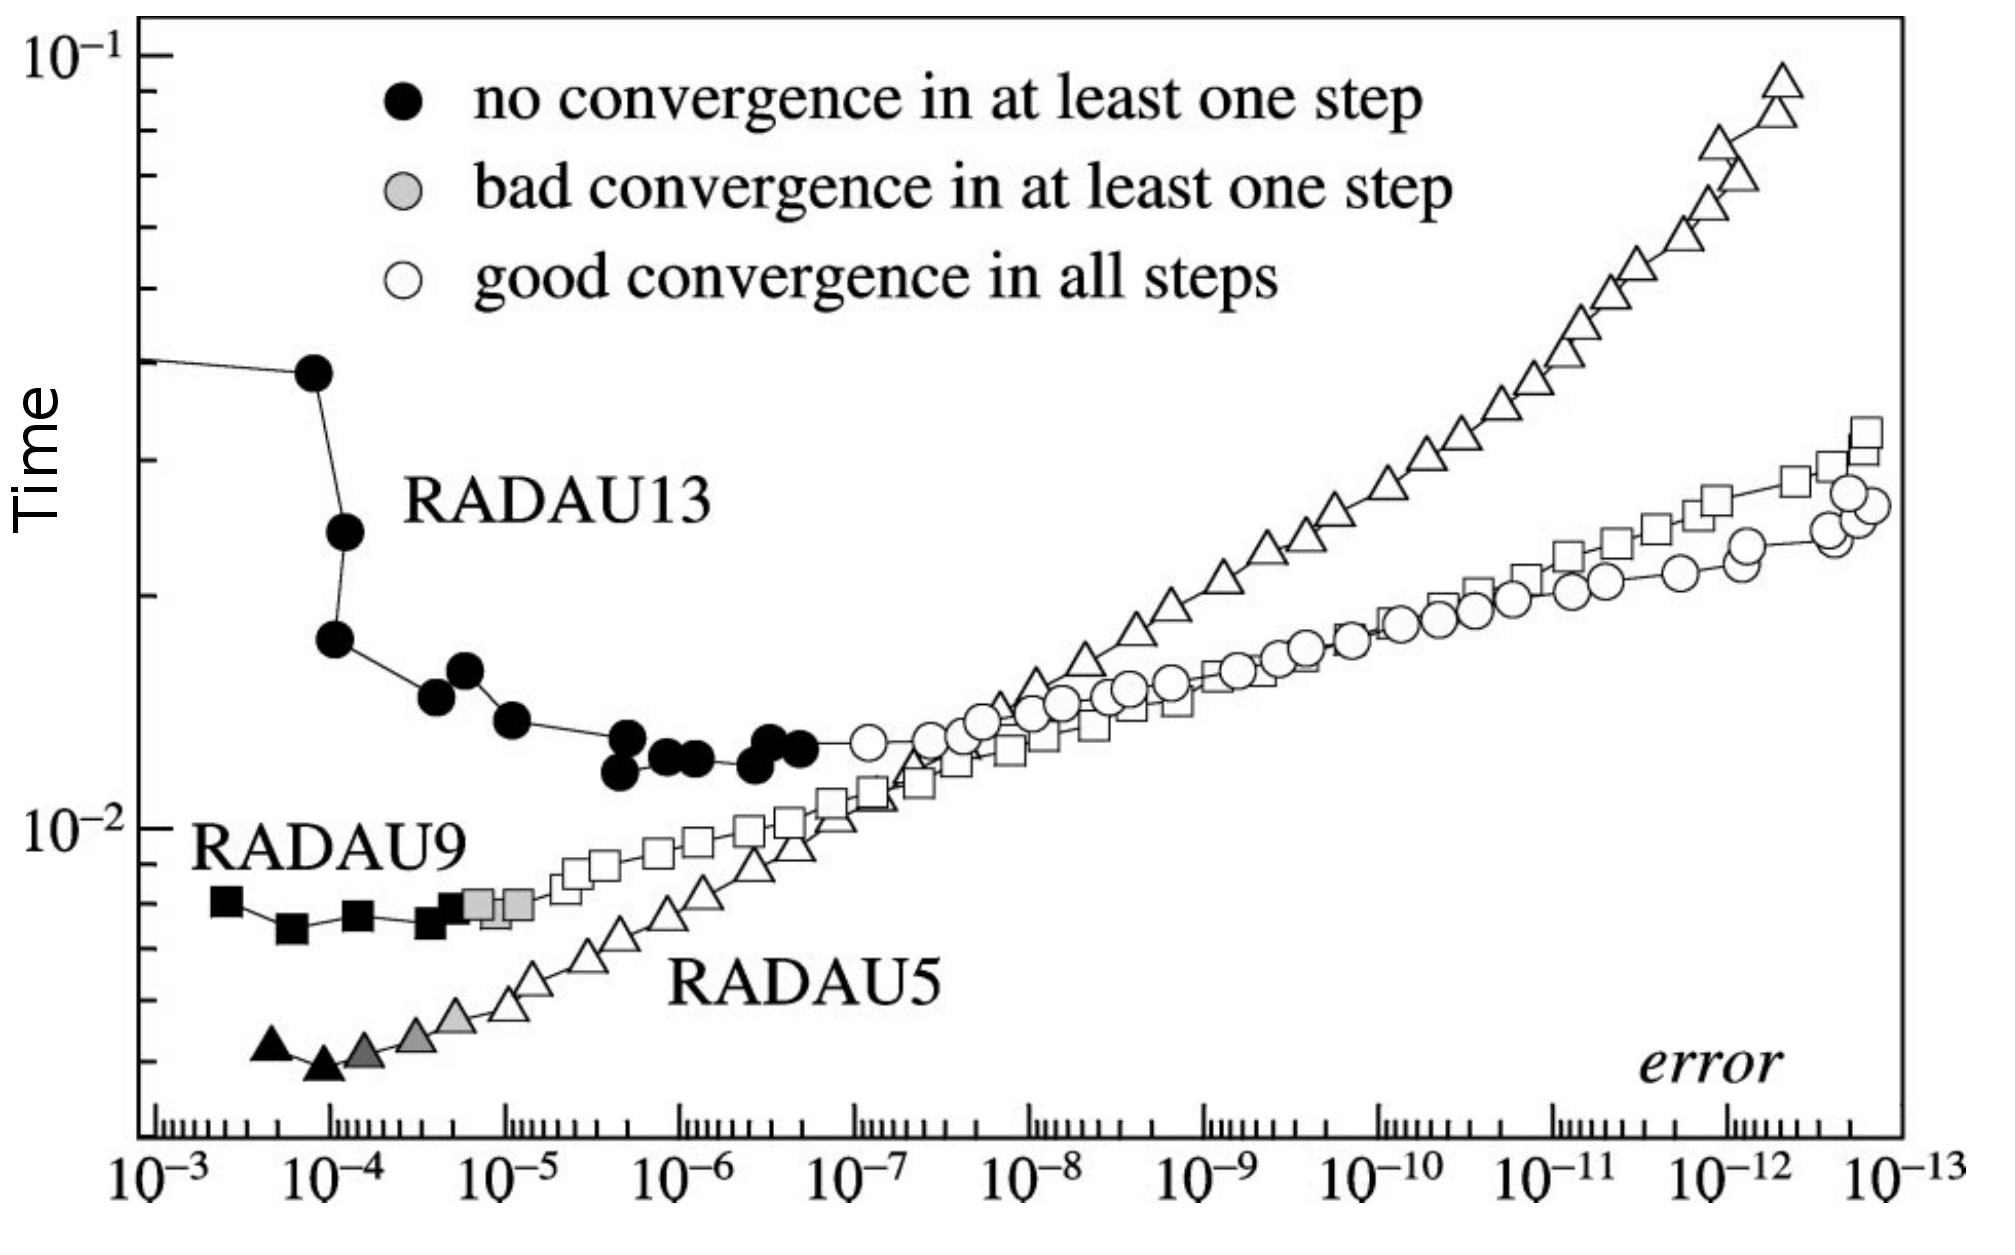
\includegraphics[width=0.8\textwidth]{figures/HairerWanner-WorkPrecision.png}\\
    {\scriptsize [Hairer and Wanner (1999)]}
  \end{center}
  \begin{itemize}
  \item Tests discretization, adaptivity, algebraic solvers, implementation
  \item No reference to number of time steps, number of grid points, etc.
  \end{itemize}
\end{frame}
